\documentclass{article}
\usepackage[brazil]{babel}
\usepackage[T1]{fontenc}
\usepackage[utf8]{inputenc}
\usepackage{graphicx}
\usepackage{times}
\usepackage{framed}
\usepackage{biblatex}
\usepackage{xcolor}
\usepackage{hyperref}

\colorlet{shadecolor}{orange!15}

\title{Laboratório 2}
\author{Leonardo Chatain}

\addbibresource{ex1.bib}

\begin{document}
\maketitle

\section{Tarefa}
Implementar o algoritmo de Dijkstra, que permite calcular o menor caminho entre um nodo e qualquer outro de um grafo. Como estrutura de heap, foi utilizada uma \emph{Árvore de Van Emde Boas}, logo a complexidade do Dijkstra é $O((m + n) \log\log n)$. Validar experimentalmente que o desempenho é $O((m + n) \log\log n)$. Determinar a constante de proporcionalidade $c$, tal que o tempo é $c*(m + n) \log\log n$.

\section{Solução}
Implementei o algoritmo de Dijkstra usando um heap de Van Emde Boas, como visto em aula. Heaps de Van Emde Boas realizam as operações \emph{insert} - no código: \emph{push(T val)} -, \emph{deletemin} - no código: \emph{pop()} -, e \emph{update} - no código: \emph{update(T val, T new)} com complexidade $ \log n $ (onde \emph{n} é o número de vértices do grafo).

Para o desenvolvimento foi utilizada a linguagem C++ e o compilador gcc versão 4.6. Para os testes foi utilizado o framework CppUnit.

\section{Ambiente de teste}

Os resultados foram obtidos utilizando-se um \emph{Intel core i7}, com um processador de $2.27$ GHz e $8$ GB de RAM.

Para os testes do algoritmo de Dijkstra foram utilizados grafos gerados randomicamente de tamanho $n=11264 + i * 1024, i = 1, 2, \ldots, 6$. Todos os grafos utilizados eram completos, ou seja, o número de arestas $m=n ^ 2$

Cada teste foi repetido $10$ vezes e foi tomada a média dos tempos de execução.

\section{Resultados}

\subsection{Heap de Van Emde Boas}

A complexidade das operações \emph{insert}, \emph{deletemin} e \emph{update} é $ \log\log n $.

Para executar os testes, fizeram-se $ n $ repetidas operações ao heap de tamanho $ n $ (n inserts, n deletemins, n updates), o que ao todo tem uma complexidade de $ n \log\log n $

A Figura~\ref{fig1} mostra o tempo de execução da operação \emph{insert}, com complexidade $\log\log n$ executada $n$ vezes. A Figura~\ref{fig2} mostra o tempo de execução da operação \emph{insert}, dividido pela complexidade teórica $n * \log\log n$.

Podemos perceber que a complexidade teórica não parece ser correspondida pela implementação. Um possível motivo para isso é que o tamanho de n é muito baixo.

\begin{figure}
  \centering
  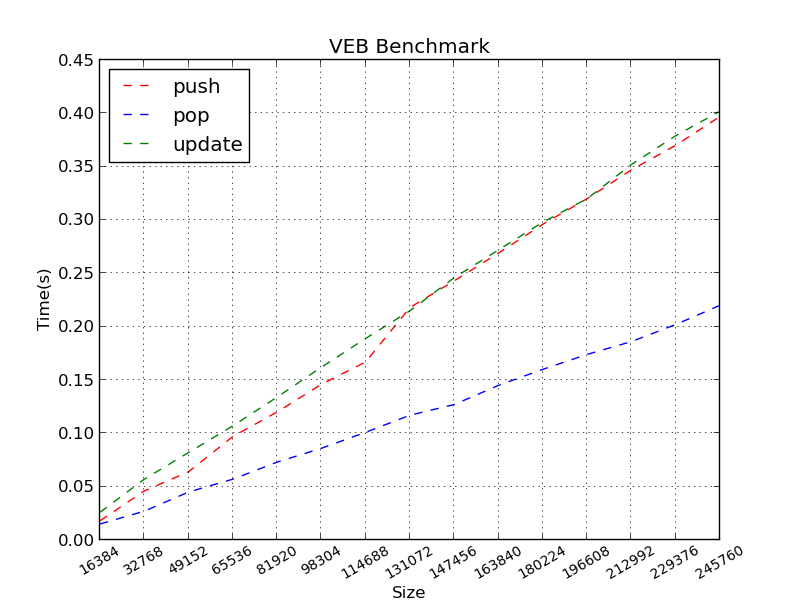
\includegraphics[width=\textwidth,keepaspectratio]{heap2.png}
  \caption{Tempo de execução $T_o$ das operações de insert, deletemin e update em um Heap de Van Emde Boas.}
  \label{fig1}
\end{figure}

\begin{figure}
  \centering
  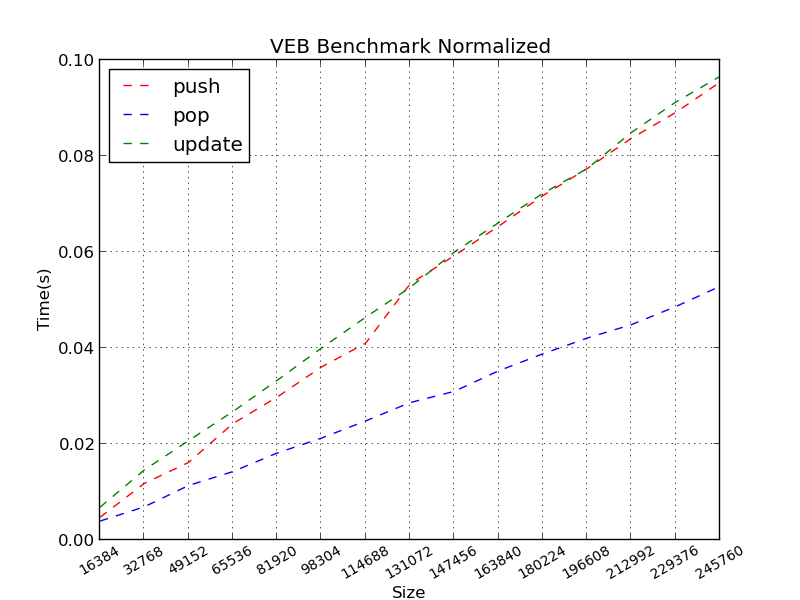
\includegraphics[width=\textwidth,keepaspectratio]{heap_inv2.png}
  \caption{Tempo de execução $T_o$ das operações de insert, deletemin e update em um Heap de Van Emde Boas, dividido pela complexidade teórica $\log\log n$}
  \label{fig2}
\end{figure}


\subsection{Dijkstra}

Como mencionado anteriormente, todos os grafos utilizados são completos, portanto $m=n^2$ e a complexidade do algoritmo é $(n^2 + n) \log\log n$.

Para executar os testes, fizeram-se 10 queries aleatórias a grafos completos de tamanhos variados.

A Tabela~\ref{tab1} mostra o tempo de execução do algoritmo de Dijkstra para um grafo completo com $n=11264 + i * 1024, i = 1, 2, \ldots, 6$ vértices e $n ^ 2$ arestas.


\begin{table}
  \centering
  \begin{tabular}{rrrrrrrrrrrrrr}
    \hline
    n =             & 512  & 1024 & 1536 & 2048 & 2560 & 3072        \\
    $T_o$ [$s$]     & 0.021 & 0.088 & 0.198 & 0.293 & 0.496 & 0.653     \\
    \hline
    n =             & 3584 & 4096  & 4608 & 5120  & 5632  & 6144  \\
    $T_o$ [$s$]     & 0.813 & 1.32  & 1.631 & 2.031 & 2.517 & 2.804 \\
    \hline
    n =             & 6656  & 7168  & 7680  & 8192  \\
    $T_o$ [$s$]     & 0.957 & 3.792 & 4.622 & 3.731 \\
    \hline
  \end{tabular}
  \caption{Tempo de execução $T_o$ do algoritmo de Dijkstra para um grafo completo com $n=11264 + i * 1024, i = 1, 2, \ldots, 6$ vértices e $n ^ 2$ arestas.}
  \label{tab1}
\end{table}

O gráfico do tempo de execução é plotado na Fig.~\ref{fig1}.

\begin{figure}
  \centering
  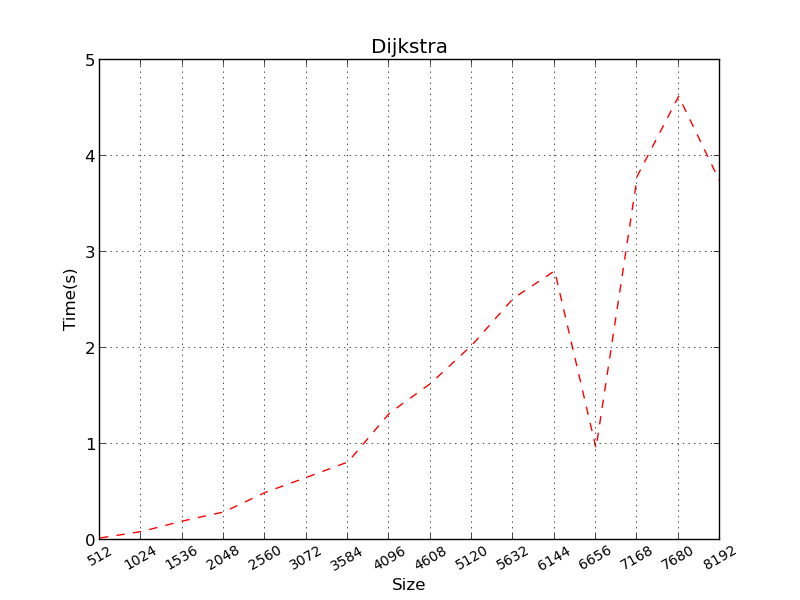
\includegraphics[width=\textwidth,keepaspectratio]{dij2.png}
  \caption{Tempo de execução $T_o$ do algoritmo de Dijkstra para um grafo com $n=11264 + i * 1024, i = 1, 2, \ldots, 6$ vértices e $n ^ 2$ arestas.}
  \label{fig3}
\end{figure}

A Fig.~\ref{fig4} mostra o gráfico do tempo de execução normalizado $T_o/(n^2+n)\log\log n$. Podemos ver que o gráfico se aproxima de uma reta para valores grandes de n.
\begin{figure}
  \centering
  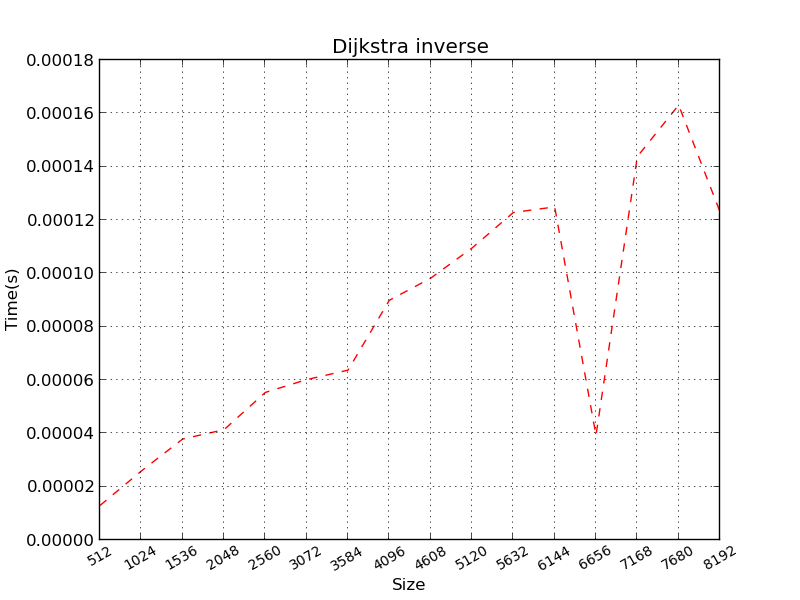
\includegraphics[width=\textwidth,keepaspectratio]{dij_inv2.png}
  \caption{Tempo de execução normalizado $T_o/(n^2+n)\log\log n$ do algoritmo de Dijkstra para um grafo com $n=11264 + i * 1024, i = 1, 2, \ldots, 6$ vértices e $n ^ 2$ arestas.}
  \label{fig4}
\end{figure}

\section{Comparando com um Heap Binomial}
O Heap Binomial é na prática mais eficiente que o Heap de Van Emde Boas. Isso corresponde ao resultado esperado, visto que o overhead de gerenciar uma árvore de Van Emde Boas é muito grande perto do ganho não significativo de um fator $\log$ a mais (podemos pensar que o primeiro $\log$ reduz em muito o tempo final, e o segundo muito pouco).

A Fig.~\ref{fig5} mostra a comparação dos tempos de execução do algoritmo de Dijkstra com um heap binário e com um heap de Van Emde Boas.


\begin{figure}
  \centering
  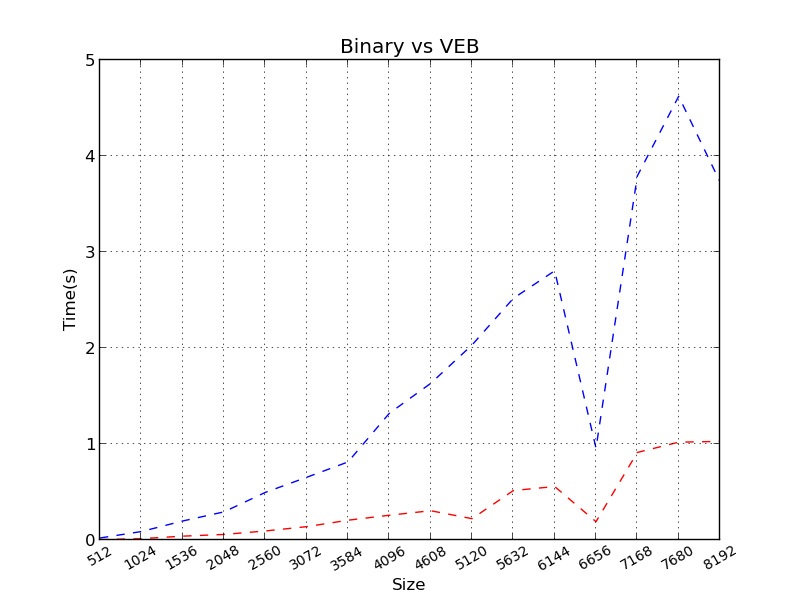
\includegraphics[width=\textwidth,keepaspectratio]{ex1_ex2.png}
  \caption {Comparação entre os tempos de execução do algoritmo de Dijkstra com um heap binário e com um heap de Van Emde Boas.}
  \label{fig5}
\end{figure}


\section{Conclusão}

A complexidade não equivale à esperada, provavelmente porque o tamanho da entrada não é grande o suficiente ($\log\log n$ provavelmente requer um tamanho grande na entrada para produzir uma diferença relevante no tempo.

Também pudemos notar que Van Emde Boas é muito mais lento que um heap binário na prática, em grande parte devido à alta complexidade da estrutura de Van Emde Boas. Outro fator interessante é que o segundo $\log$ nos ganha muito pouco com relação ao primeiro $\log$, e isso é provavelmente suficiente para que uma estrutura $\log\log$ não valha a pena.

\printbibliography

\end{document}
% Local Variables:
% auto-fill-function: do-auto-fill
% TeX-PDF-mode: t
% fill-column: 110
% ispell-local-dictionary: "brasileiro"
% mode-name: "LaTeX"
% End:
